\documentclass[a4paper,10pt]{article}
\usepackage[spanish]{babel}
\usepackage{hyperref}
\usepackage[pdftex]{graphicx}
\usepackage{amsfonts}
\usepackage{amsmath}
\usepackage{verbatim}
\usepackage[utf8]{inputenc}
\usepackage{./paquetes/newalgo}

\hypersetup{
  pdftitle={Algoritmos y Estructura de Datos III - Trabajo Práctico 1},
  colorlinks,
  citecolor=black,
  filecolor=black,
  linkcolor=black,
  urlcolor=black 
}

%opening
\makeatletter 

\def\materia#1{\def\Materia{#1}}
\def\tptit#1{\def\tptit{#1}}
\def\subtit#1{\def\subtit{#1}}
\def\res#1{\def\res{#1}} %variable res
\def\integrantes#1{\def\integrantes{ {\sffamily {\fontsize{10pt}{0pt} #1} }} }

\def\keyvar#1{\def\keyvar{#1}}

\newcommand{\Res}[1]{
	\begin{abstract}
		\vspace*{-1mm}
		#1
	\end{abstract}
}

\newcommand{\keywords}[1]{
	\begin{center}
		{\footnotesize \textbf{Keywords} \vskip 4pt #1 }
	\end{center}
}


% Carátula
\renewcommand{\maketitle}{
	\begin{titlepage}
		\vspace*{-100pt}
		\let\footnotesize\small
		\let\footnoterule\relax
		\parindent \z@
		\reset@font
		\null\vfil

		\vskip 10\p@
		\hbox{
			\vrule depth 0.9\textheight
			\mbox{\hspace{2em}}
			\vtop{
				\vskip 30\p@
				\begin{center}
					\textsf{Universidad de Buenos Aires} \\
					\textsf{Facultad de Ciencias Exactas y Naturales} \\
					\textsf{Departamento de computación} \\
				\end{center}
	
				\vspace{10pt}
	
				% Título
				\begin{center}
					{\sffamily {\Large \tptit}}
				\end{center}
	
				% Subtítulo
				\begin{center}
					{\sffamily {\textbf{\huge \subtit}}}
				\end{center}
	
				\par
				\hrule height 2pt
				\par
				\begin{center}
					{\fontsize{10pt}{0pt} {
						\sffamily Joaquín Garavaglia - LU 28/08 - yjuaco@hotmail.com
 						\par Matías Barbeito - LU 179/08 - matiasbarbeito@gmail.com
						\par Santiago Pivetta - LU 318/08  - pive\_86@gmail.com       
						\par Mariano Semelman - LU 143/08 - marianosoy@gmail.com }
					} \par
				\end{center}
				\vskip 30\p@

	
				% Abstract
				\Res{\res}
				\vskip 10\p@
				% Keywords
				\keywords{\keyvar}

				\vfill
				\vspace*{0mm}

	
				\begin{minipage}[t]{\textwidth}
			%        \begin{minipage}[t]{.55 \textwidth}
			%            \includegraphics{logo_uba.jpg}
			%        \end{minipage}
					\hspace*{-7mm}
				\end{minipage}
			}
		}
 
	\end{titlepage}
	\setcounter{footnote}{0}
}


%%%%%%%%%%%%%%%%%%%%%%%%%%%%%%%%%%%%%%%%%%%%%%%%%%%%%%%%%%%%%%%%%%%%%%%%%%%


%\makeatother
\tptit{Algoritmos y Estructuras de datos III }
\subtit{Trabajo Práctico I}

\res{
\indent  \\
\indent
}


%\keyvar{} % palabras claves


\begin{document}

\maketitle
\tableofcontents
\setlength{\parskip}{0.2cm}

\newpage
\section{Introducción general}

\newpage
\section {Ejercicio 1}
\subsection{Introducción}
En este ejercicio se pide que, dados ciertos pasillos que unen una determinada cantidad de habitaciones, y sabiendo que algunas contienen puertas y otras llaves para abrirlas, ver si es posible llegar de la primera a la última habitación (es decir de la \textit{1} a la \textit{n}). \\
Este problema claramente se puede modelar con un grafo, donde cada habitación es un nodo que puede contener una puerta, una llave (la cual abre una única puerta) o nada, y cada pasillo es una arista. \\
Luego, resolver el ejercicio pedido es equivalente a ver si se puede llegar al nodo \textit{n} (donde \textit{n} es la cantidad de nodos) partiendo desde el \textit{1}. Esto debe hacerse teniendo en cuenta que es necesario pasar por algunos nodos como requisito para pasar por otros (hay que conseguir la llave correspondiente a cada puerta).
En las siguientes secciones explicaremos en detalle el modelo y el algoritmo utilizado para resolver el problema, y también analizaremos la complejidad del mismo.


\subsection{Explicación}
Nuestra heurística constructiva se basa en una idea de densidades dentro del grafo y consiste en orientar la búsqueda del clique máximo priorizando las zonas de mayor densidad.
Experimentamos con 2 medidas diferentes de densidad, definidas como $\delta$1 y $\delta$2, 
que son asignadas a cada nodo antes de comenzar el algoritmo.
Definimos $\displaystyle \delta$1 para el nodo i  como el promedio de los grados de todos sus vecinos y de el mismo ,

   $\displaystyle \delta1(i) = \frac{\sum_{j=1,j-vecino-i}^{n} grado(j) + grado(i)}{grado(i)+1} $

Por otro lado definimos $\displaystyle \delta$2 para el nodo i como la suma de los grados de todos sus vecinos y de el mismo. 
	
   $\displaystyle \delta2(i) = {\sum_{j=1,j-vecino-i}^{n} grado(j) + grado(i)}$

En un principio pensamos el $ \delta2(i)$ sin embargo consideramos que había casos en los que la suma de los grados de los nodos vecinos no nos orientaba bien hacia cliques máximos, podría caer a explorar nodos con muchos vecinos(tipo estrella) pero que no formaban cliques, por lo tanto surgió la idea del $ \delta1(i)$ con el que probamos en primer lugar.
Este tiene la particularidad de que incluye en el promedio el grado del nodo actual, con lo cual dados dos nodos con igual promedio entre sus vecinos (por ej uno con 1 solo vecino de grado 3 y otro con 10 vecinos de grado 3)prioriza al que tiene mayor grado (el de 10). 
Sin embargo luego de hacer corridas con ambos deltas, observamos que si bien salvábamos esos casos, había otros en los que era mejor utilizar el  $ \delta2(i)$ ,tal como se puede observar en la tabla de resultados.

Una vez calculadas las densidades de todos los nodos, tomamos el nodo de mayor densidad y empezamos la búsqueda del cliqué máximo que contiene a ese nodo,insertándolo en el conjunto solución Cq e insertando a todos sus vecinos en una cola de prioridad S(prioridad de máxima densidad).
La cola de prioridad S contendrá durante todo el algoritmo a todos los candidatos posibles a formar parte del cliqué obtenido hasta el momento Cq.
Una vez vacía S el algoritmo termina, en el peor caso el cliqué máximo es el grafo completo y todos los nodos son en algún momento insertados en S y luego quitados e insertados en Cq.

\begin{verbatim}
generarDensidad()										O(n*n)
	
merge(nodo i,S,Cq)										O(n*log(|Cq|))	        
     para todo w vecino de i 
        si(w no esta en Cq y no fue encolado en S)
          encolar w en S
fin

expandirClique(Cq,S)								
    mientras S no vacía					 			
        w=tope de S									
        Si esClique(w,Cq)       O(|Cq|)				
            insertar w en Cq    O(log(|Cq|))  } * O(n) = O(n*n*log(|Cq|)) = O(n*n*log(n)))
            merge(w,S,Cq)       O(n*log(|Cq|))		
        desencolar w de S		              
fin												
									
HC()										 	
    generarDensidad()           O(n*n)		   	
    insertar nodoMax en Cq      O(1)            } = O (n*n*log(n)) 	
    merge(NodoMax,S,Cq)         O(n)			   
    expandirClique(Cq,S)        O(n*n*log(n))	 	
fin												

\end{verbatim}
La función merge itera en peor caso sobre n-1 vecinos y para cada uno pregunta si está en Cq ,lo cual tiene un costo de log(|Cq|) según referencia de la función count de set de STL. 
Podemos observar que la complejidad de la función expandirClique determina que el peor caso para el algoritmo HC es el grafo completo, ya que la misma itera sobre el conjunto S de los candidatos sin repetir hasta que éste quede vacío; en cada iteración, Cq aumenta en uno (w) y se mergean los vecinos de w a S.
La complejidad nos queda expresada así ,donde i es el tamaño de Cq que se va incrementando en cada interación y los 3 terminos de la sumatoria corresponden a las funciones esClique,insertar y merge dentro del ciclo

$\displaystyle \sum_{i=1}^{n} i + log(i) + n*log(i) <= \frac{n(n-1)}{2}+\sum_{i=1}^{n} (n+1)*log(i) <=$  
 
$\displaystyle  <= \frac{n(n-1)}{2}+(n+1)*log(i!) <= \frac{n(n-1)}{2}+(n+1)*n*log(n) $

Luego la complejidad de HC es O(n*n) + O(1) + O(n) + O(n*n*log(n)) = O(n*n*log(n))  



\subsection{Detalles de implementación}
El ejercicio compila con el comando \texttt{make} .\\
El algoritmo recibe como parámetros de entrada tres nombres de archivo \emph{'entrada'},\emph{'salida'} y \emph{'tiempos'}, y se ejecuta \texttt{./secuencias entrada.in salida.out tiempos.times}.\\
El archivo \emph{'entrada'} (.in) contiene una lista de secuencias de enteros cada secuencia en una línea precedida de su longitud y el fin de la lista lo determina una línea con -1.\\
El archivo \emph{'salida'} (.out)lo genera el algoritmo con los resultados de cada secuencia(cantidad de mínima de elementos a eliminar de la secuencia tal que la subsecuencia resultante sea unimodal).\\
Por último el archivo \emph{'tiempos'} (.times)  también generado por el algoritmo, contendrá una tabla con el tamaño de cada secuencia y tiempo de ejecución correspondiente, para cada una.\\
La generación de secuencias 'entrada' se realizó con un generador de secuencias(véase\\ \texttt{generador\_de\_secuencias/generador\_secuencias.cpp}), éste compila con el comando make y se ejecuta con 
\texttt{./secuencias modo archivo\_entrada.in  min max escala}, donde modo debe ser r=random(no implementamos otro), archivo entrada.in es el nombre del archivo donde va a volcar la lista de secuencias generada, min es el valor mínimo de tamaño de secuencia, max es el máximo y escala la diferencia de tamaño entre secuencias conjuntas a generar en la lista.\\
El generador genera secuencias de Naturales, no de Enteros pero consideramos que a efectos experimentales el comportamiento es el mismo para números negativos, de todas formas se realizaron tests para los mismos.
Agregar el parámetro escala tanto como min y máx fue necesario, ya que en un principio, al probar con secuencias de menos de 20 elementos, e incrementando a escalas pequeñas no se observaba claramente la relación cuadratica de los tiempos, luego encontramos un razonable set de datos para las experimentaciones definitivas, listas de secuencias de 20 a 800 elementos incrementando de a 10, 20 y 40.  


\subsection{Pruebas y Resultados}
Se adjunta con el trabajo un script bash que se usó para correr los tests llamado \textit{test.sh}, junto con un \textit{Tp3.in} que contiene los casos de prueba usados.\\
El programa no solo informa en Tp3TS.out el resultado con el formato indicado, sino que por consola informa el tamaño del clique máximo, n, m y el tiempo más corto de 5 corridas iguales (en nanosegundos).
Para la entrega esta porción de código está comentada, pero si se quieren repetir los tests, descomentar esa parte, recompilar el tp, y correr test.sh (que guarda todo lo mostrado por consola en 
el archivo tests_resultados).

\subsection{Conclusiones}
Consideramos que los resultados hallados son buenos por tratarse de una heurística constructiva y por la dimensión de los grafos,de todas formas creemos que podría realizarse una mejora eligiendo otra función para $delta$ que tome lo favorable de cada una de las dos con las que experimentamos. 
Por otro lado nos quedarían por realizar corridas con grafos patológicos, ya que los grafos de las experimentaciones fueron en su mayoría randoms como en el caso de p-hat que es una generalización del generador de grafos randoms uniformes y ver cuan lejos de la solución óptima podemos caer. 


\newpage
\section {Ejercicio 2}
\subsection{Introducción}
En este ejercicio se pide que, dados ciertos pasillos que unen una determinada cantidad de habitaciones, y sabiendo que algunas contienen puertas y otras llaves para abrirlas, ver si es posible llegar de la primera a la última habitación (es decir de la \textit{1} a la \textit{n}). \\
Este problema claramente se puede modelar con un grafo, donde cada habitación es un nodo que puede contener una puerta, una llave (la cual abre una única puerta) o nada, y cada pasillo es una arista. \\
Luego, resolver el ejercicio pedido es equivalente a ver si se puede llegar al nodo \textit{n} (donde \textit{n} es la cantidad de nodos) partiendo desde el \textit{1}. Esto debe hacerse teniendo en cuenta que es necesario pasar por algunos nodos como requisito para pasar por otros (hay que conseguir la llave correspondiente a cada puerta).
En las siguientes secciones explicaremos en detalle el modelo y el algoritmo utilizado para resolver el problema, y también analizaremos la complejidad del mismo.


\subsection{Explicación}
Nuestra heurística constructiva se basa en una idea de densidades dentro del grafo y consiste en orientar la búsqueda del clique máximo priorizando las zonas de mayor densidad.
Experimentamos con 2 medidas diferentes de densidad, definidas como $\delta$1 y $\delta$2, 
que son asignadas a cada nodo antes de comenzar el algoritmo.
Definimos $\displaystyle \delta$1 para el nodo i  como el promedio de los grados de todos sus vecinos y de el mismo ,

   $\displaystyle \delta1(i) = \frac{\sum_{j=1,j-vecino-i}^{n} grado(j) + grado(i)}{grado(i)+1} $

Por otro lado definimos $\displaystyle \delta$2 para el nodo i como la suma de los grados de todos sus vecinos y de el mismo. 
	
   $\displaystyle \delta2(i) = {\sum_{j=1,j-vecino-i}^{n} grado(j) + grado(i)}$

En un principio pensamos el $ \delta2(i)$ sin embargo consideramos que había casos en los que la suma de los grados de los nodos vecinos no nos orientaba bien hacia cliques máximos, podría caer a explorar nodos con muchos vecinos(tipo estrella) pero que no formaban cliques, por lo tanto surgió la idea del $ \delta1(i)$ con el que probamos en primer lugar.
Este tiene la particularidad de que incluye en el promedio el grado del nodo actual, con lo cual dados dos nodos con igual promedio entre sus vecinos (por ej uno con 1 solo vecino de grado 3 y otro con 10 vecinos de grado 3)prioriza al que tiene mayor grado (el de 10). 
Sin embargo luego de hacer corridas con ambos deltas, observamos que si bien salvábamos esos casos, había otros en los que era mejor utilizar el  $ \delta2(i)$ ,tal como se puede observar en la tabla de resultados.

Una vez calculadas las densidades de todos los nodos, tomamos el nodo de mayor densidad y empezamos la búsqueda del cliqué máximo que contiene a ese nodo,insertándolo en el conjunto solución Cq e insertando a todos sus vecinos en una cola de prioridad S(prioridad de máxima densidad).
La cola de prioridad S contendrá durante todo el algoritmo a todos los candidatos posibles a formar parte del cliqué obtenido hasta el momento Cq.
Una vez vacía S el algoritmo termina, en el peor caso el cliqué máximo es el grafo completo y todos los nodos son en algún momento insertados en S y luego quitados e insertados en Cq.

\begin{verbatim}
generarDensidad()										O(n*n)
	
merge(nodo i,S,Cq)										O(n*log(|Cq|))	        
     para todo w vecino de i 
        si(w no esta en Cq y no fue encolado en S)
          encolar w en S
fin

expandirClique(Cq,S)								
    mientras S no vacía					 			
        w=tope de S									
        Si esClique(w,Cq)       O(|Cq|)				
            insertar w en Cq    O(log(|Cq|))  } * O(n) = O(n*n*log(|Cq|)) = O(n*n*log(n)))
            merge(w,S,Cq)       O(n*log(|Cq|))		
        desencolar w de S		              
fin												
									
HC()										 	
    generarDensidad()           O(n*n)		   	
    insertar nodoMax en Cq      O(1)            } = O (n*n*log(n)) 	
    merge(NodoMax,S,Cq)         O(n)			   
    expandirClique(Cq,S)        O(n*n*log(n))	 	
fin												

\end{verbatim}
La función merge itera en peor caso sobre n-1 vecinos y para cada uno pregunta si está en Cq ,lo cual tiene un costo de log(|Cq|) según referencia de la función count de set de STL. 
Podemos observar que la complejidad de la función expandirClique determina que el peor caso para el algoritmo HC es el grafo completo, ya que la misma itera sobre el conjunto S de los candidatos sin repetir hasta que éste quede vacío; en cada iteración, Cq aumenta en uno (w) y se mergean los vecinos de w a S.
La complejidad nos queda expresada así ,donde i es el tamaño de Cq que se va incrementando en cada interación y los 3 terminos de la sumatoria corresponden a las funciones esClique,insertar y merge dentro del ciclo

$\displaystyle \sum_{i=1}^{n} i + log(i) + n*log(i) <= \frac{n(n-1)}{2}+\sum_{i=1}^{n} (n+1)*log(i) <=$  
 
$\displaystyle  <= \frac{n(n-1)}{2}+(n+1)*log(i!) <= \frac{n(n-1)}{2}+(n+1)*n*log(n) $

Luego la complejidad de HC es O(n*n) + O(1) + O(n) + O(n*n*log(n)) = O(n*n*log(n))  



\subsection{Detalles de implementación}
El ejercicio compila con el comando \texttt{make} .\\
El algoritmo recibe como parámetros de entrada tres nombres de archivo \emph{'entrada'},\emph{'salida'} y \emph{'tiempos'}, y se ejecuta \texttt{./secuencias entrada.in salida.out tiempos.times}.\\
El archivo \emph{'entrada'} (.in) contiene una lista de secuencias de enteros cada secuencia en una línea precedida de su longitud y el fin de la lista lo determina una línea con -1.\\
El archivo \emph{'salida'} (.out)lo genera el algoritmo con los resultados de cada secuencia(cantidad de mínima de elementos a eliminar de la secuencia tal que la subsecuencia resultante sea unimodal).\\
Por último el archivo \emph{'tiempos'} (.times)  también generado por el algoritmo, contendrá una tabla con el tamaño de cada secuencia y tiempo de ejecución correspondiente, para cada una.\\
La generación de secuencias 'entrada' se realizó con un generador de secuencias(véase\\ \texttt{generador\_de\_secuencias/generador\_secuencias.cpp}), éste compila con el comando make y se ejecuta con 
\texttt{./secuencias modo archivo\_entrada.in  min max escala}, donde modo debe ser r=random(no implementamos otro), archivo entrada.in es el nombre del archivo donde va a volcar la lista de secuencias generada, min es el valor mínimo de tamaño de secuencia, max es el máximo y escala la diferencia de tamaño entre secuencias conjuntas a generar en la lista.\\
El generador genera secuencias de Naturales, no de Enteros pero consideramos que a efectos experimentales el comportamiento es el mismo para números negativos, de todas formas se realizaron tests para los mismos.
Agregar el parámetro escala tanto como min y máx fue necesario, ya que en un principio, al probar con secuencias de menos de 20 elementos, e incrementando a escalas pequeñas no se observaba claramente la relación cuadratica de los tiempos, luego encontramos un razonable set de datos para las experimentaciones definitivas, listas de secuencias de 20 a 800 elementos incrementando de a 10, 20 y 40.  


\subsection{Pruebas y Resultados}
Se adjunta con el trabajo un script bash que se usó para correr los tests llamado \textit{test.sh}, junto con un \textit{Tp3.in} que contiene los casos de prueba usados.\\
El programa no solo informa en Tp3TS.out el resultado con el formato indicado, sino que por consola informa el tamaño del clique máximo, n, m y el tiempo más corto de 5 corridas iguales (en nanosegundos).
Para la entrega esta porción de código está comentada, pero si se quieren repetir los tests, descomentar esa parte, recompilar el tp, y correr test.sh (que guarda todo lo mostrado por consola en 
el archivo tests_resultados).

\subsection{Conclusiones}
Consideramos que los resultados hallados son buenos por tratarse de una heurística constructiva y por la dimensión de los grafos,de todas formas creemos que podría realizarse una mejora eligiendo otra función para $delta$ que tome lo favorable de cada una de las dos con las que experimentamos. 
Por otro lado nos quedarían por realizar corridas con grafos patológicos, ya que los grafos de las experimentaciones fueron en su mayoría randoms como en el caso de p-hat que es una generalización del generador de grafos randoms uniformes y ver cuan lejos de la solución óptima podemos caer. 


\newpage
\section{Ejercicio 3}

\subsection{Explicación}

El algoritmo luego de parsear 'entrada' y convertir cada string hora en  int, guarda los datos  en una \emph{$lista< Planilla*>$},donde Planilla es \emph{$vector<int>$}. (Esto lo realiza la función parsearInstancias(string s),ver \texttt{src/parser.cpp} ).Cada Planilla contiene en la primera mitad de los datos las horas de entrada de todos los programadores y en la segunda mitad las horas de salida .
\newline
Una vez hecho ésto, comienza el ciclo principal del algoritmo al cual le tomamos el tiempo usando la clase Timer (ver \texttt{include/timer.h} y \texttt{src/timer.cpp}),que devuelve el resultado expresado en nanosegundos .
\newline
El ciclo principal  itera sobre la \emph{$lista<Planillas*>$}  y  está representado por la función maxCant(Planilla* p), que es la que realiza el cálculo principal sobre cada Planilla.
\newline
Básicamente maxCant itera simultáneamente sobre los subvectores de cada Planilla, entrada(comienza en el index=0) y salida (comienza en index= planilla.size()/2) y realiza el conteo de programadores que estan en simultáneo en cada momento .

Un pseudocódigo de ésto sería : 
\begin{verbatim}
 para toda planilla p de la lista <Planillas*> list  hacer{
               prender el  timer;                                    O(1)
               calcular maxCant(Planilla* p)                         O(maxCant(p))
               guardar resultado en string res                       O(1)
  }
  
 maxCant(Planilla* p) { 
     inicializo variables                                             O(1)
     aux =0,res=0;		
     mientras no haya recorrido todas las entradas de p{              O(p.size())
            mientras no haya recorrido todas las entradas de p y 
            la hora de entrada actual sea menor a la hora de salida actual{
		  
                     aux++ ;
                     proxima entrada;		
	        }
            si  (aux > res){res = aux}
            mientras no haya recorrido todas las entradas de p y 
            la hora de salida actual es menor a la hora de entrada actual{
			   
                      aux--;				 	
                      proxima salida,
            }
     }	
	 devuelvo res 
  }
	  
\end{verbatim}
Podemos observar un ciclo mientras, que contiene dos subciclos mientras, éstos son los encargados de hacer el merge de las dos sublistas de entrada y salida, el primero hace entrar a todos los programadores antes de que salga alguno incrementando aux y el segundo lo mismo, hace salir a todos los programadores antes de que entre alguno decrementando aux. 
\newline
Luego de cada ciclo de entradas,se chequea si el aux superó al res anterior, guardando siempre la máxima cantidad de programadores que estuvieron en simultáneo en la oficina, es importante aclarar que con éste algoritmo, estamos contando al programador que se va de la oficina en un instante dado  como incluído dentro de la cantidad de programadores en ese instante, por eso el primer ciclo cuenta las entradas y las prioriza a las salidas aunque se hagan en el mismo instante .
\newline
Claramente se observa que la cantidad de operaciones es lineal al tamaño de la planilla, ya que por cada entrada o salida de la planilla se ejecuta una cantidad constante de operaciones en alguno de los dos subciclos, por lo cual utilizamos el modelo uniforme para el cálculo de la complejidad y decimos que la complejidad del algoritmo es lineal al tamaño de la entrada (O(p.size()).
\newline
Podríamos considerar un mejor caso en el que por ejemplo si  todos ingresaran antes de que el primero egrese, el algoritmo realizaría p.size()/2 iteraciones de entrada y ninguna de salida, ya que no nos interesan las salidas una vez que terminaron de ingresar todos, pero de todas formas la complejidad sigue siendo del orden de p.size() por una constante (1/2), o sea lineal al tamaño de la planilla(entrada del algoritmo).
\newline 
Respecto de un peor caso, podríamos considerar uno en el que los ingresos y egresos sean alternados uno a uno, de ésta manera el ciclo sería  1) evaluar el mientras ppal, 2)  iterar 1 vez  el mientras de entradas, 3) iterar 1 vez el mientras de salida  y asi sucesivamente, haciendo que  por cada dos elementos de la planilla, se realizan 3 iteraciones de ciclo (cada uno con una cantidad constante de operaciones), sin embargo, la complejidad sigue teniendo el mismo orden (sería p.size()*3/2 que es O(p.size()).


\subsection{Detalles de implementación}
El ejercicio compila con el comando \texttt{make} .
\newline
El algoritmo recibe como parámetros de entrada tres nombres de archivo \emph{'entrada'},\emph{'salida'} y \emph{'tiempos'}, y se ejecuta \texttt{./planillas entrada.in salida .out tiempos.times}
\newline
El archivo \emph{'entrada'} (.in) contiene un conjunto de listas (llamadas planillas en el algoritmo) de las horas de  entradas y salidas de los programadores.
\newline
El tamaño de cada planilla es de  2*cantidad de programadores, donde la primera mitad de horas corresponde a las entradas (ordenadas de menor a mayor ) y la segunda mitad corresponde a las salidas también ordenadas .
\newline
El archivo \emph{'salida'} (.out)lo genera el algoritmo con los resultados de cada planilla  (cantidad de programadores que se encuentran en simultáneo en la oficina).
\newline
Por último el archivo \emph{'tiempos'} (.times)  también generado por el algoritmo, contendrá una tabla con el tamaño de la planilla y tiempo de ejecución correspondiente, para cada instancia .
\newline
La generación de planillas 'entrada' se realizó con un generador de planillas (véase \texttt{generador\_de\_planillas/generador\_planillas.cpp} ), éste compila con el comando make y se ejecuta con 
./planillas modo archivo\_entrada.in  min max escala, donde modo puede ser r=random, w=worst o peor caso, archivo entrada.in es el nombre del archivo donde va a volcar la lista de planillas, min es el valor mínimo de tamaño de planilla, max es el máximo y escala la diferencia de tamaño entre planillas conjuntas en la lista a generar .
\newline
Agregar el parámetro escala tanto como min y máx fue necesario, ya que en un principio, al probar con planillas de menos de 200 datos, e incrementando a escalas pequeñas no se observaba claramente la relación lineal de los tiempos, luego encontramos un razonable set de datos para las experimentaciones definitivas, listas de planillas de 200 a 2000 programadores (o sea de 400 a 4000 datos) incrementando de a 50 .  

\subsection{Pruebas y Resultados}

Una vez elegidos los valores representativos para la generación de lotes de planillas, se realizaron 3 lotes Random de listas de planillas (véase \texttt{rand\_200\_2000\_50.in}, \texttt{rand2\_200\_2000\_50.in}, \texttt{rand3\_200\_2000\_50.in} ) y se calcularon los tiempos de ejecución del algoritmo, obteniendo los resultados en los respectivos .out y las tablas de tiempos en los .times, con las que se obtuvieron los siguientes gráficos.
\newline
\newline
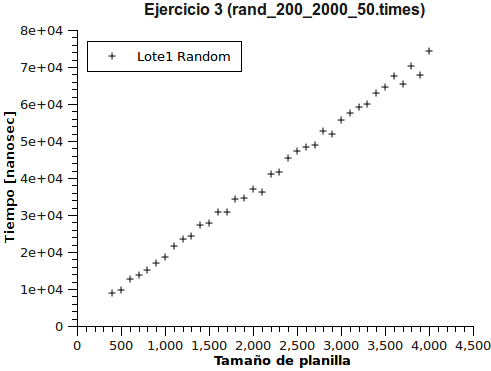
\includegraphics[scale=0.8]{Graph1.png}
\newline
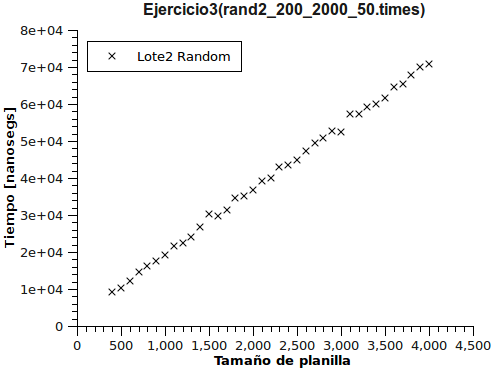
\includegraphics[scale=0.8]{Graph2.png}
\newline
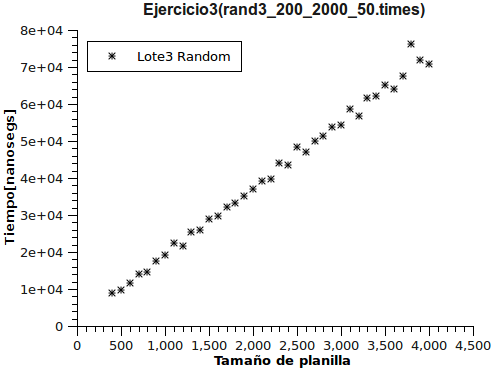
\includegraphics[scale=0.8]{Graph3.png}
\newline


Por otro lado se realizó un lote Worst o Peor caso,(véase \texttt{worst\_200\_2000\_50.in}) y se obtuvo el siguiente gráfico de la tabla de tiempos .

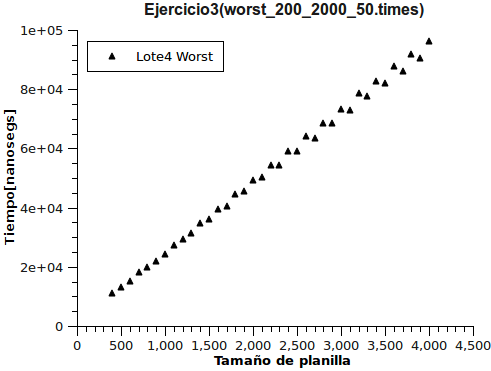
\includegraphics[scale=0.8]{Graph4.png}





\subsection{Conclusiones}

Como era de esperar, el gráfico nos describe una función aproximadamente lineal, observamos que en el que consideramos el peor caso, la pendiente de la 'cuasi recta' es mas pronunciada que en los casos randoms o casos promedio,se puede observar que alcanza valores del orden de $10^{5}$ para planillas de 4000 datos, contra los de orden de $10^{4}$ de los lotes randoms para el mismo tamaño de datos. 
\newline
Sin embargo a los efectos del cálculo de la complejidad, ésto no hace diferencia, ya que la diferencia está dada por una constante multiplicativa .





\end{document}
